\chapter{Approach}
In this section we will describe our approach and enumerate problems that we encountered.

\section {Compiling Broadway and C-Breeze}

As described in the previous section, we wanted to get an updated and compiled version of the Broadway annotations language. A compiled version of Broadway would help us understand the dependencies and interaction of the annotations with Broadway and C-Breeze.  The original Broadway was built upon GCC 2.95. We found that it took a fair amount of work and fixes to get the original Broadway code to compile with a newer version of GCC (4.2). In addition, we had to make corrections to C-Breeze as well, since Broadway relied on C-Breeze's internal structures. One major problem we encountered was utilizing the GNU \textit{Flex}\footnote{http://flex.sourceforge.net/} and \textit{Bison}\footnote{http://www.gnu.org/software/bison/} to actually generate the language tokens and parser for the Broadway's annotation language. Therefore, we spent time learning Flex and Bison, in order to modify the original grammar for changes to support the latest version of both programs.  In the end, we had a compiled version of Broadway that could parse annotations, but a bug that we were never able to resolve hindered the original Broadway from performing its actual analysis. Even without a fully functional Broadway compiler, this enabled us to start lifting annotation code out, since it was at least being properly parsed.

\section {Decoupling C-Breeze}

We knew that completely decoupling C-Breeze from our ported annotation language was important, but the task proved to be nearly impossible without rewriting the annotation language (parser and tokenizer) and annotations analyzer over again. Our main goal here was to remove the C-Breeze compiler dependencies, so that we could make use of the arbitrary C-code in annotation files with LLVM. 

\subsection{Isolate Annotation Code}
Our first attempt to decouple annotation code was to simply pull out the individual annotation classes relevant to parsing and analyzing purely annotations. However, we discovered that within the grammar, C-Breeze structures were utilized by Broadway in the \textit{actions} of grammar rules (non-terminals). This was because an Abstract Syntax Tree (AST) identical to C-breeze's AST was built using C-Breeze structures as c-statements were being parsed by Broadway's annotation parser.  Therefore, the next logical step was to just to isolate annotations rules and tokens that do not interact with the C-grammar. 

The problem here was that the C-grammar was not only used to parse arbitrary C-code that could be given in the annotations through code replacements, but it actually used to parse conditions and most importantly parse the header C-blocks. The header C-blocks are used to declare the procedures that are annotated and the structures created from the rest of the file depend heavily on their definitions. Here is a reminder of an Annotation file's structure:

\begin{enumerate}
\item  C-code blocks: include native C code, including header files and other declarations.
\item Properties: attributes that define flow values for library-specific dataflow analysis.
\item Procedures: Information for routines in the library interface, including the dependence information, pointer behavior, and its effects on object properties.
\item Global variables:  global variables that  can represent hidden or abstract state information.
\end{enumerate}

In our work, we are primarily concerned with the Properties and Procedures. However, the original Broadway Annotation class required the C-code blocks in order to do preprocessing and learning about the procedures. After analyzing the C-code grammar, we determined it was not reasonable to rewrite and debug the C-code grammar in the given time due to its complexity and importance to the Annotation's class. Therefore, we made a compromise to remove a portion of C-Breeze dependencies. 

\subsection{Narrow Scope and Remove C-code replacement}
We decided to not support \textit{C-code replacement}. We need C-code parsing to learn about the header, but we found we could minimize the interactions with the actual C-Breeze compiler if we did not allow C-code replacement. This is because C-code replacement would actually require C-Breeze to build an AST and compile it into a IR. 
In addition, the C-Breeze IR and LLVM IR are different, so we could not directly use the original C-Breeze generated IR in our LLVM pass. However, even with these changes, we needed to use the C-Breeze AST data structures since they were interwoven with the grammar and Broadway's Annotation class. Later, we will explain how we use these data structures, but made a lot of modifications to access more of the raw information to do our own logic and analysis.

We briefly looked into exploring a way to turn C-Breeze AST to LLVM IR or LLVM supported AST, but a properly functioning translator would take up too much time. Given our extensive sifting through the dependencies of the old Broadway Annotation class and the C-Breeze compiler, we would suggest future projects to rewrite subsets of the annotation language to conform to the structure of the target compiler opposed to a full conversion that we initially attempted.

\begin{figure*}[t!]
\begin{center}
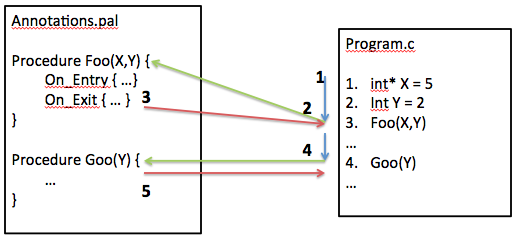
\includegraphics[width=0.75\textwidth]{interface}
\caption{This shows the general interaction of the Broadway IDFA and pointer Analysis. The  \textit{blue} lines indicates the normal data-flow analysis. The \textit{green} lines show where a library function is hit, and a request is made to the \textit{ProceducureAnnotationInfo} about the library function. The \textit{red} lines indicate the information returned to the analysis driver.  }
\label{fig:interface}
\end{center}
\end{figure*}

\section{Interface for IDFA and Pointer Analysis}

After we successfully had a running \textit{Annotations} parsing class, we needed to provide an interface that the Iterative Data-Flow Analysis (IDFA) and Pointer Analysis could call such that it could request annotation information about a procedure. Information that is apparently relevant are the variables and memory blocks coming into the procedure, those thats get modified, those that are accessed, and those that come out of the procedure. Therefore, we implemented several classes to provide this support. 

\begin{itemize}
\item {\bf Annotations} : This class holds all the parsed \textit{.pal} file.
\item {\bf AnnotationPass} : This class implements LLVM's \textit{ModulePass} and simply takes in an annotation file (\textit{.pal}) as a parameter and then constructs an \textit{Annotations} object and \textit{ProceducureAnnotationInfo} object. 
\item {\bf ProceducureAnnotationInfo} : This class provides methods to query the Annotations object's data structures for information such as \textit{getEntry, getExit, uses, and defs}
\end{itemize}

Figure \ref{fig:interface} shows a simple outline of how the IDFA and pointer analysis would interact with the annotations. As information is needed, the IDFA driver would use the ProceducureAnnotationInfo object to query information it is interested in. These classes will also be used in our annotation analysis described in the following section.


\section{Library-Level Error Detection}

The final usage of our annotations is to perform annotation analysis. In particular, we decided to focus on library-level Error Detection as described in Sam Guyer's thesis \citep{bdwythesis}. By removing the compiling dependencies on C-Breeze, the Annotations class could not actually do original annotations analysis found in the original Broadway code. Therefore, we had to write our own logic and interpretation of the annotations.  We decided that we wanted to focus on solving was a subset of interesting cases from the Broadway grammar, in particular Library-level Error Detection. The main idea behind this  type of analysis is to identify places in a program where library calls are used incorrectly or unsafely, and then push this information to the surface. In order to perform this analysis, we implemented the {\bf ClientProblem} interface specified by the IDFA work done by another group. We implemented the {\bf AnnotationAnalaysis} class. This class provides call-backs to our annotation analysis whenever particular statements are reached during the IDFS and pointer analysis. In particular, we were interested every time a library function was called. The ClientProblem interface currently provides different types of call-backs, and we found it currently efficiently supports a flow-insensitive annotation analysis. Therefore, we focused on flow-insensitive error detection. We tackled two main approaches for identifying vulnerabilities or errors.

\subsection{Enum Properties and Data Flow Values}\label{sec:enumprops}
The first approach is to use {\bf properties} to propagate data flow values of attributes we care about. For example, we could care about format string vulnerability problems. In this case, if a string is modified by an unsafe source, we would like to propagate a property value of \textit{taintedness} around. Therefore, if any piece of code references the \textit{tainted} memory block, it would be good to know. The primary driver for this approach is an {\bf enum property} from the annotation language. The enum property  enumerates a set of hierarchal properties that get assigned to memory blocks. The general pipeline is as follows:

\begin{enumerate}
\item An annotation file defines a set of property values for a specific property of interest. \item Then for relevant procedures in the library, annotations are written to assign property values to memory blocks as conditions or met. These values are associated with memory blocks and are propagated with the data-flow analysis. 
\item As the IDFA proceeds through the program, a corresponding \textit{meet} operator is applied on each property value at \textit{meet} points, and our AnnotationAnalysis object stores this information. 
\item In the end, the AnnotationAnalysis objects summarizes its findings for each memory blocks.
\end{enumerate}

In the \textit{taintedness} example, the final output for each memory block would be if the block is \textit{tainted, untainted, or could be either}.

\subsection{Errors Reports Analysis}
Our second approach is error and analysis rules based on conditions. We use a subset of the conditions grammar to support conditions involving enum properties. We only support a subset of conditions here. Many complex conditions are handled by the C-code grammar and C-Breeze compiler which we tried to avoid. Error analysis follows similar steps as described in Section \ref{sec:enumprops}. However, rather than actually holding values that are propagated through the data-flow analysis, it simply outputs to a log or stream what ``effects" (characteristics) it has found. For example, given an identifier (memory block) we can determine if conditions are met by traversing the property value lattice. If we return to our ``taintedness" example, suppose we asked if a memory block ``could be" \textit{tainted}. If true, we could report an error or warning at that point in the program. This information can be consumed by the client to understand simple conditions are being met or violated.
 
